Modellbildung der Strecke durch mathematische Beschreibungen der Wirkungszusammenh�nge zwischen den Systemgr��en, die f�r die Aufgabenstellung relevant sind.

Ein Modell ist eine aufgabenspezifische Vereinfachung der Realit�t. In der RT bew�hrte Modellierungsform:

\section{Darstellung der Strecke als Strukturbild (Blockschaltbild)}
\subsection{Beispiel: Permanten erregter Gleichstrommotor}
\begin{itemize}
	\item Ger�teschema: (siehe Beiblatt 4)
	\item Systemdarstellung:
\end{itemize}

\begin{center}
	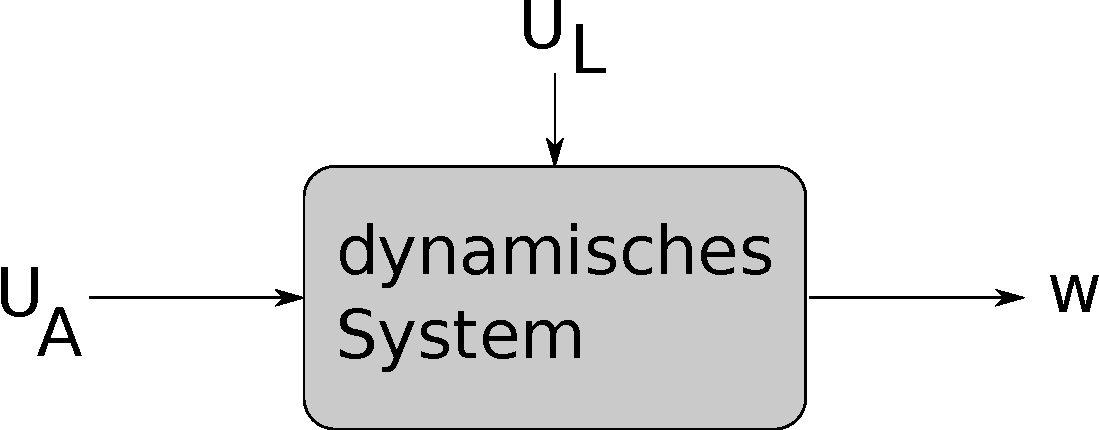
\includegraphics[width=200px]{graphics/gleichstrommotor.pdf}
\end{center}

\subsubsection{Ermittlung der beschreibenden Gleichungen}

\begin{equation}
  u_l(t) = L \frac{di_a} {dt} \longrightarrow \frac{d i_a(t)}{d t} = \frac{1}{L_A} u_l(t) \longrightarrow
\end{equation}
\begin{equation}
  i_a(t) = i_a(0) + \frac{1}{L_A} \int_0^t u_l{\tau}, d\tau
\end{equation}


